% !TEX TS-program = pdflatex

\documentclass[a4paper,11pt,oneside,onecolumn]{article}
\usepackage[english]{babel}
\usepackage{graphicx}
\usepackage{psfrag}
\usepackage{amstext,epsfig,amssymb,amsbsy,amsmath}
\usepackage{bm}
\usepackage{caption}
\usepackage{subcaption}
%\usepackage[latin1]{inputenc}
\usepackage{sectsty}
\usepackage[margin=1in,headheight=13.6pt]{geometry}
\allsectionsfont{\sffamily}
\usepackage{fancyhdr}
\pagestyle{fancy}
\fancyhf{}
%\fancyhead[RE,RO]{}
%\fancyhead[RE,LO]{Guides and tutorials}
\fancyhead[LE,LO]{CUT}
\fancyfoot[RE,RO]{Page \thepage}
\renewcommand{\headrulewidth}{1pt}
\renewcommand{\footrulewidth}{1pt}
\selectlanguage{english}
\usepackage[shortlabels]{enumitem}
\usepackage{titlesec}
\newcommand{\ua}{\underline{a\!}\,}
\usepackage{steinmetz}
\usepackage{mdframed}
\usepackage{pifont}
\usepackage{float}
\usepackage[linktoc=all]{hyperref}
\hypersetup{
	colorlinks,
	citecolor=black,
	filecolor=black,
	linkcolor=black,
	urlcolor=black
}
\usepackage{multicol}
\usepackage{booktabs}
\usepackage{rotating}

\usepackage[makeroom]{cancel}


\newenvironment{warning}
{\par\begin{mdframed}[linewidth=2pt,linecolor=red]%
		\begin{list}{}{\leftmargin=1cm
				\labelwidth=\leftmargin}\item[\Large\color{red}\ding{43}]}
		{\end{list}\end{mdframed}\par}
	
\newenvironment{hint}
{\par\begin{mdframed}[linewidth=2pt,linecolor=blue]%
		\begin{list}{}{\leftmargin=1cm
				\labelwidth=\leftmargin}\item[\Large\color{blue}\ding{45}]}
		{\end{list}\end{mdframed}\par}
	
%% Units
\usepackage[
per-mode=fraction,
detect-all,
detect-display-math = true,
detect-inline-family = text, %% NEEDS CURRENT VERSION OF SIUNITX
detect-inline-weight = text
]{siunitx}
% some specific power system units (which are not standard SI units..)
\DeclareSIUnit\pu{pu}
\DeclareSIUnit\voltampere{VA}
\DeclareSIUnit\var{var}
% define the versor notation ('1<5?'). Usage \versor[unit]{magnitude}{angle}
\newcommand{\versor}[3][]{#2\phase{#3^\circ}\,\si{#1}}

\usepackage{tikz}
\usetikzlibrary{shapes, arrows, arrows.meta}
\usetikzlibrary{decorations.pathreplacing}
\usetikzlibrary{positioning}
\usetikzlibrary{decorations.pathmorphing}
\usetikzlibrary{decorations.mypathmorphing}
\usetikzlibrary{decorations.markings}
\usetikzlibrary{patterns}
% DO NOT INPUT ANY CIRCUITS LIBRARIES HERE; AS THERE IS A CLASH BETWEEN
% circuitikz and circuits
\usetikzlibrary{circuits, circuits.ee.IEC}
\usepackage[europeanresistors,americaninductors,smartlabels]{circuitikz}
%\input{../circuitsPowerSystemSymbols.sty}
% \usepackage[european]{circuitikz}
\usepackage{pgfplots}
% Load the library
%\usetikzlibrary{external}
% Enable the library !!!>>> MUST be in the preamble <<<!!!!
%\tikzexternalize

\usepackage{ifthen}
\newboolean{student-version}  
\newcommand{\mysolution}[1] {%
	\ifthenelse{\boolean{student-version}}{}{%
		\subsection*{Solution}
		#1%
		\newpage
	}%
}

\newcommand{\myexercise}[2] {%
		\subsection{#1}
		#2%
}

\usepackage{xsim}
\xsimsetup{
	%  exercise/within=chapter,
	% exercise/template=theorem ,
	exercise/within = section ,
	exercise/the-counter = \thesection.\arabic{exercise} ,
	%  exercise/the-counter=\thechapter.\arabic{exercise},
	path = {temp}
}

\DeclareExerciseProperty{exhint}
% we'll use a description list for the hints:
\newcommand\printexhints{%
	\begin{description}
		\ForEachUsedExerciseByType{%
			\def\ExerciseType{##1}%
			\def\ExerciseID{##2}%
			\GetExercisePropertyT{exhint}
			{%
				\item[\XSIMmixedcase{\GetExerciseName}~##3]
				####1%
			}%
		}%
	\end{description}
}

\newcommand\exhint[1]{\SetExerciseProperty{exhint}{#1}}


\DeclareExerciseProperty{exanswer}
% we'll use a description list for the answers:
\newcommand\printexanswers{%
	\begin{description}
		\ForEachUsedExerciseByType{%
			\def\ExerciseType{##1}%
			\def\ExerciseID{##2}%
			\GetExercisePropertyT{exanswer}
			{%
				\item[\XSIMmixedcase{\GetExerciseName}~##3]
				####1%
			}%
		}%
	\end{description}
}

\newcommand\exanswer[1]{\SetExerciseProperty{exanswer}{#1}}


\def\begs{\begin{split}}
\def\ends{\end{split}}
\def\begequ{\begin{equation}}
\def\endequ{\end{equation}}
\def\lab{\label}
\def\begdes{\begin{description}}
\def\enddes{\end{description}}
\def\begenu{\begin{enumerate}}
\def\begite{\begin{itemize}}
\def\endite{\end{itemize}}
\def\endenu{\end{enumerate}}
\def\ctscale{0.7}
\def\ctlinewidth{0.5pt}

\gappto{\UrlBreaks}{\UrlOrds}
%%% Greek 
\usepackage[utf8]{inputenc}
%\usepackage[greek,english]{babel}
\usepackage{alphabeta} 
\usepackage[gen]{eurosym}
\usepackage{listings}

\graphicspath{}

\newcounter{taskcounter}
\stepcounter{taskcounter}
\newcommand{\newtask}[1]{\subsubsection*{Task \arabic{taskcounter} [#1]}%
	\stepcounter{taskcounter}%
}

\rhead{\leftmark}
\lfoot{Last updated: \today}

\usepackage{upquote}
\usepackage{fancyvrb}

\newcommand\textcode{\Verb}


\begin{document}
\begin{titlepage}
	
	
\includegraphics[width=\textwidth]{SPS_logo}\par\vfill
	
	\centering 
	{\scshape\Large [EEN452] Control and Operation of Electric Power Systems\par}
	{\huge\bfseries Dynamic simulation of a five-bus system\par}
	\vspace{2cm}
	{\Large\itshape Dr~Petros Aristidou\par}
	\vspace{0.5cm}
	\textit{Sustainable Power Systems Lab\\Department of Electrical Engineering,\\Computer Engineering \& Informatics\\\url{https://sps.cut.ac.cy}}
	
	\vfill
	
	% Bottom of the page
	{\large Last updated: \today\par}
\end{titlepage}
\thispagestyle{empty}
\pagenumbering{arabic}

\tableofcontents{}

\clearpage

\section{Introduction}

This exercise is complementary to the teaching material of the course EEN452 Control and Operation of Electric Power Systems. It will help you better understand:
\begin{itemize}
	\item The behavior of the synchronous generator during system dynamics and faults.
	\item The purpose of governors, their models, and the impact to the system frequency.
	\item The purpose of AVRs, their models, and the impact to the system voltage.
	\item The purpose of PSS, their models, and the impact to the system oscillatory behavior.
	\item How to perform dynamic simulations to analyze the security of power systems.
\end{itemize}

This exercise has been heavily based on teaching material provided by Prof. Thieery Van Cutsem\footnote{\url{https://thierryvancutsem.github.io/}}.

\subsection{Grading and deliverables}

\begin{enumerate}
	\item This assignment counts for 10\% of the final grade.
	\item You must use PyRAMSES \footnote{\url{https://pyramses.sps-lab.org/}} and the online platform of the lab\footnote{\url{https://sps.cut.ac.cy/jhub}}. You can use the example exercise\footnote{\url{https://sps.cut.ac.cy/jhub-5-bus}} as the starting point.
	\item The deliverables are to be submitted are:
	\begenu
	\item A report addressing all the questions detailed in the assignment (\textbf{in PDF format}).
	\item The JupyterNotebook (ipynb file) with the student implementation with all the files needed to execute the UC problem.
	\item[*] You can instead submit everything in a \textbf{single} ipynb file, making use of the Markdown cells to answer the questions instead of submitting a separate PDF.
	\endenu
	\item Delayed submissions will be penalized by 2\% reduction for every delayed day.
	\item Any signs of plagiarism will be penalized with 0\%.
	\item If the ipynb code does not execute on the lab server, then the report will not be accepted and will be marked with 0\%.
\end{enumerate}

\section{System model}

\begin{figure}[H]
	\centering
	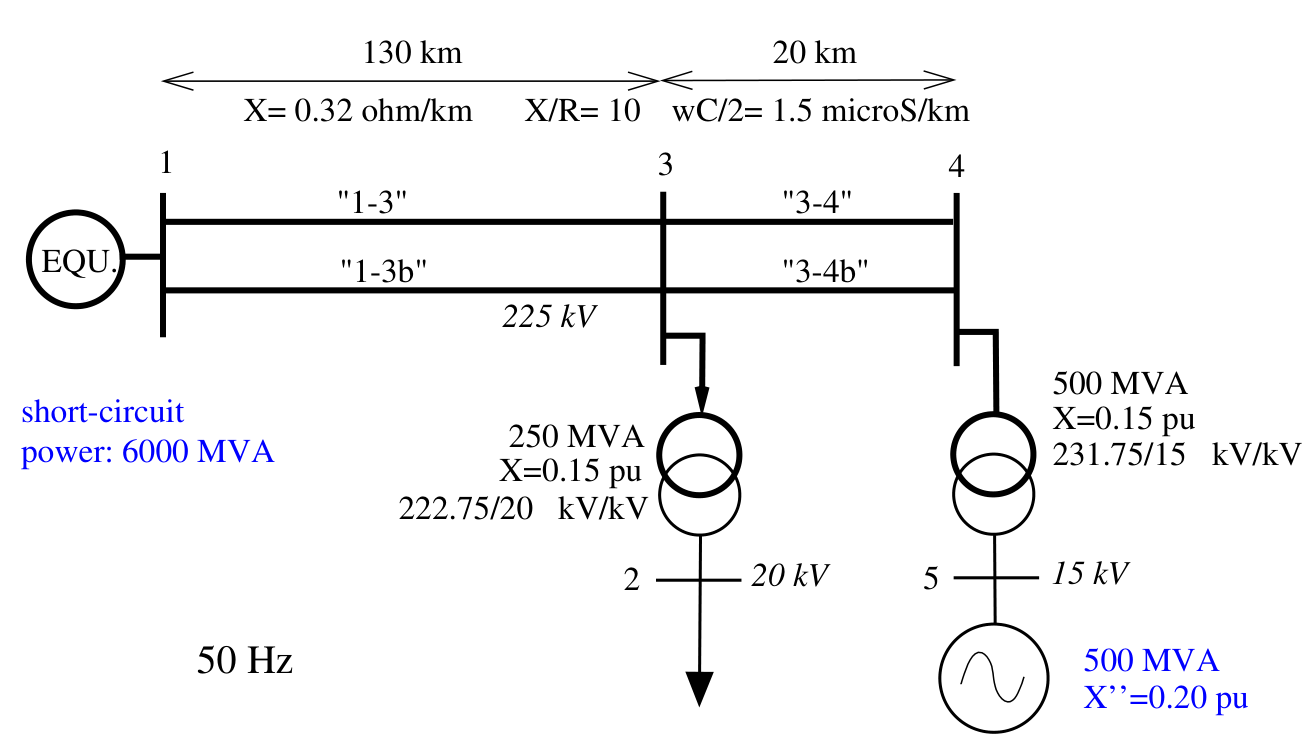
\includegraphics[width=\linewidth]{model}
	\caption{Five-bus system oneline diagram}
	\label{fig:model}
\end{figure}

\subsection{Generator at bus 5: synchronous machine data}

The synchronous machine is modeled as detailed in class\footnote{\url{https://sps.cut.ac.cy/courses/een452/sync_mac_model.pdf}}.

$$
\begin{gathered}
	R_a=0 . \quad X_{\ell}=0.15 p u \quad m=0.10 \quad n=6.0257 \\
	X_d=2.20 \quad X_d^{\prime}=0.30 \quad X_d^{\prime \prime}=0.20 p u \\
	X_q=2.00 \quad X_q^{\prime}=0.40 \quad X_q^{\prime \prime}=0.20 p u \\
	T_{d o}^{\prime}=7.00 \quad T_{d o}^{\prime \prime}=0.05 \quad T_{q \circ}^{\prime}=1.50 \quad T_{q \circ}^{\prime \prime}=0.05 \mathrm{~s} \\
	H=4 \mathrm{~s}
\end{gathered}
$$
(values in pu on the generator 500 MVA base)


\subsection{Generator at bus 5: speed governor and steam turbine}

\begin{figure}[H]
	\centering
	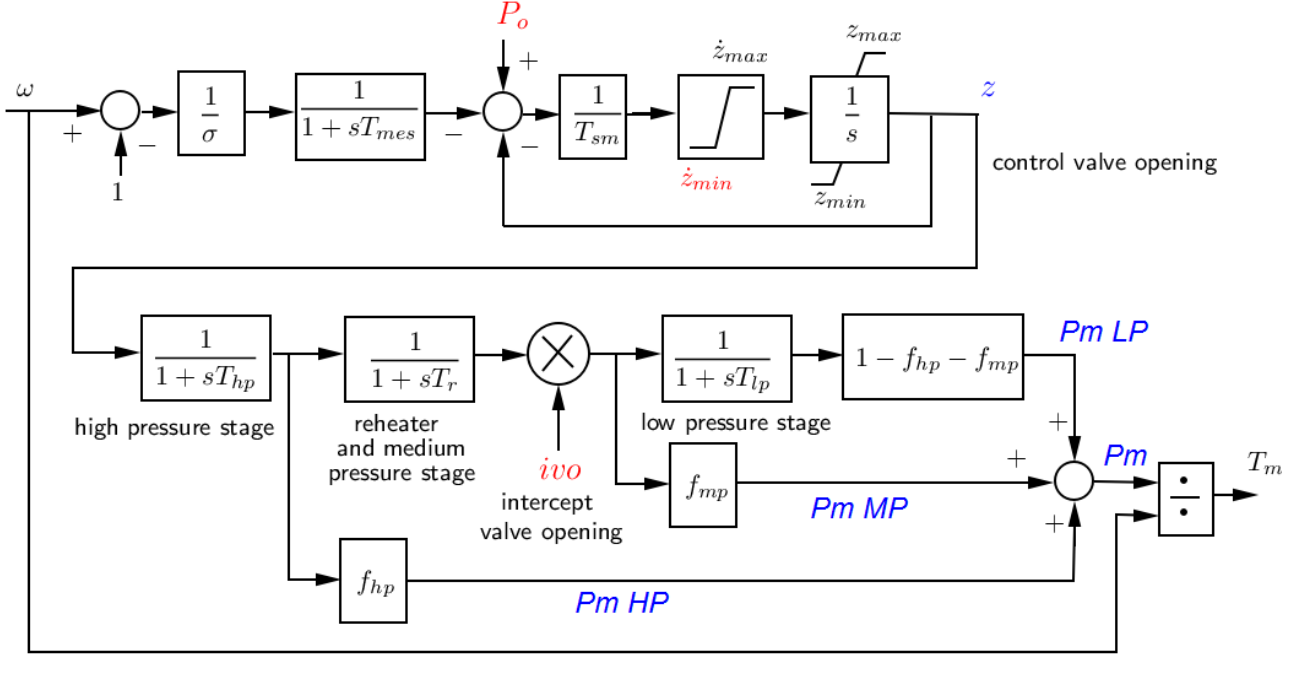
\includegraphics[width=1\linewidth]{governor}
	\caption{Speed governor}
	\label{fig:governor}
\end{figure}

$$
\begin{gathered}
	P_{nom}=460\ MW \quad \sigma=0.04 \quad T_{m e s}=0.1 \mathrm{~s} \quad T_{s m}=0.4 \mathrm{~s} \\
	\dot{z}_{\text {min }}=-0.05 \mathrm{pu} / \mathrm{s} \quad \dot{z}_{\max }=0.05 \mathrm{pu} / \mathrm{s} \quad z_{\min }=0 . \quad z_{\max }=1 . \mathrm{pu} \\
	T_{h p}=0.3 \mathrm{~s} \quad f_{h p}=0.4 \quad T_r=5.0 \mathrm{~s} \quad f_{m p}=0.3 \quad T_{l p}=0.3 \mathrm{~s} \quad \text { ivo }=1
\end{gathered}
$$

\subsection{Generator at bus 5: automatic voltage regulator, excitation system, overexcitation limiter}

\begin{figure}[H]
	\centering
	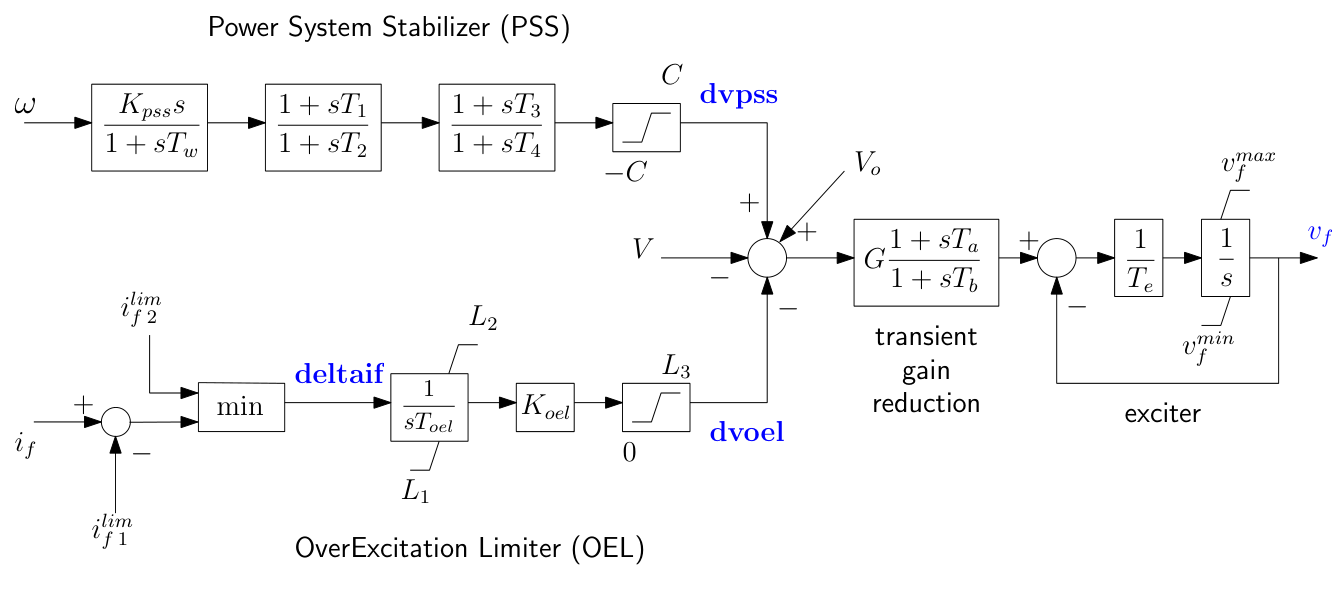
\includegraphics[width=1\linewidth]{AVR}
	\caption{Automatic voltage regulator, excitation system, overexcitation limiter}
	\label{fig:avr}
\end{figure}

$$
\begin{gathered}
	G=70 . \quad T_a=T_b=1 \mathrm{~s} \quad T_e=0.4 \mathrm{~s} \quad v_f^{\min }=0 . \quad v_f^{\max }=5 \mathrm{pu} \\
	K_{p s s}=50 \quad T_w=5 \mathrm{~s} \quad T_1=T_3=0.323 \mathrm{~s} \quad T_2=T_4=0.0138 \mathrm{~s} \quad C=0.06 \mathrm{pu} \\
	i_{f 1}^{\text {lim }}=2.90 \mathrm{pu} \quad i_{f 2}^{\text {lim }}=1.00 \mathrm{pu} \quad T_{o e l}=8 \mathrm{~s} \quad K_{o e l}=2.0 \\
	L_1=-1.1 \quad L_2=0.1 \quad L_3=0.2 \mathrm{pu}
\end{gathered}
$$

\subsection{Load tap changer controlling voltage at bus 2}

\begin{itemize}
	\item transformer ratio: $\left[0.88, 1.20\right]$
	\item number of tap positions: 33
	\item voltage dead-band: $\left[V^o-0.01 V^o+0.01\right] pu$
	\item delay before first tap change: 25 s
	\item delay between subsequent tap changes: 10 s
\end{itemize}

\subsection{Load model at bus 2}

\begin{figure}[H]
	\centering
	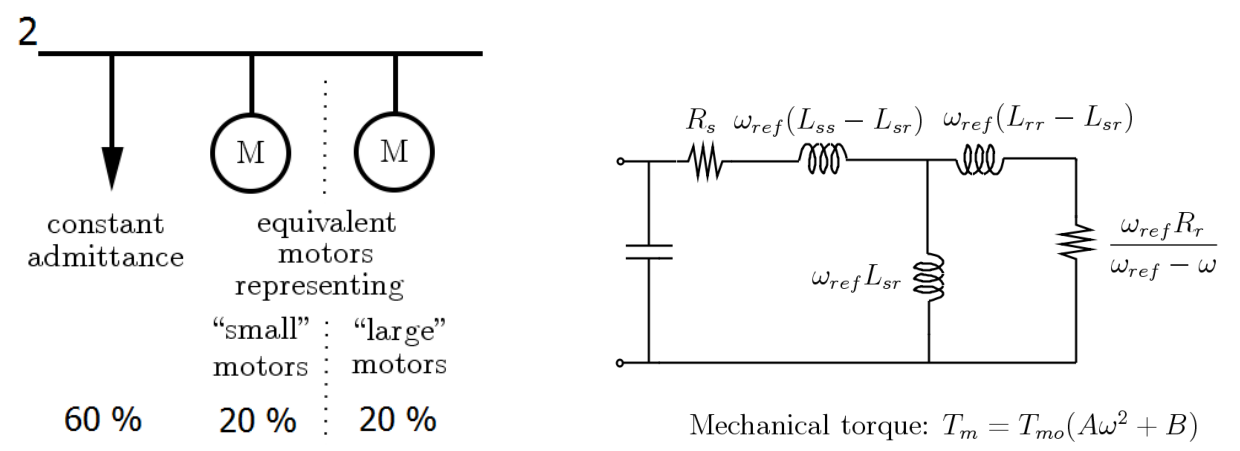
\includegraphics[width=1\linewidth]{load}
	\caption{Load model}
	\label{fig:load}
\end{figure}

\textbf{``small motors":}
$$
\begin{gathered}
	R_s=0.031 \quad L_{s s}=3.30 \quad L_{s r}=3.20 \quad L_{r r}=3.38 \quad R_r=0.018 \mathrm{pu} \\
	H=0.7 \mathrm{~s} \quad A=0.5 \quad B=0.5
\end{gathered}
$$
\textbf{``large motors":}
$$
\begin{gathered}
	R_s=0.013 \quad L_{s s}=3.867 \quad L_{s r}=3.80 \quad L_{r r}=3.97 \quad R_r=0.009 \mathrm{pu} \\
	H=1.5 \mathrm{~s} \quad A=0.5 \quad B=0.5
\end{gathered}
$$

(values in pu on the motor MVA base)

\section{Operating points}

\subsection{Operating point 1}

The first operating point assumes the generator is covering the consumption of the load and exports power to the grid.

\begin{figure}[H]
	\centering
	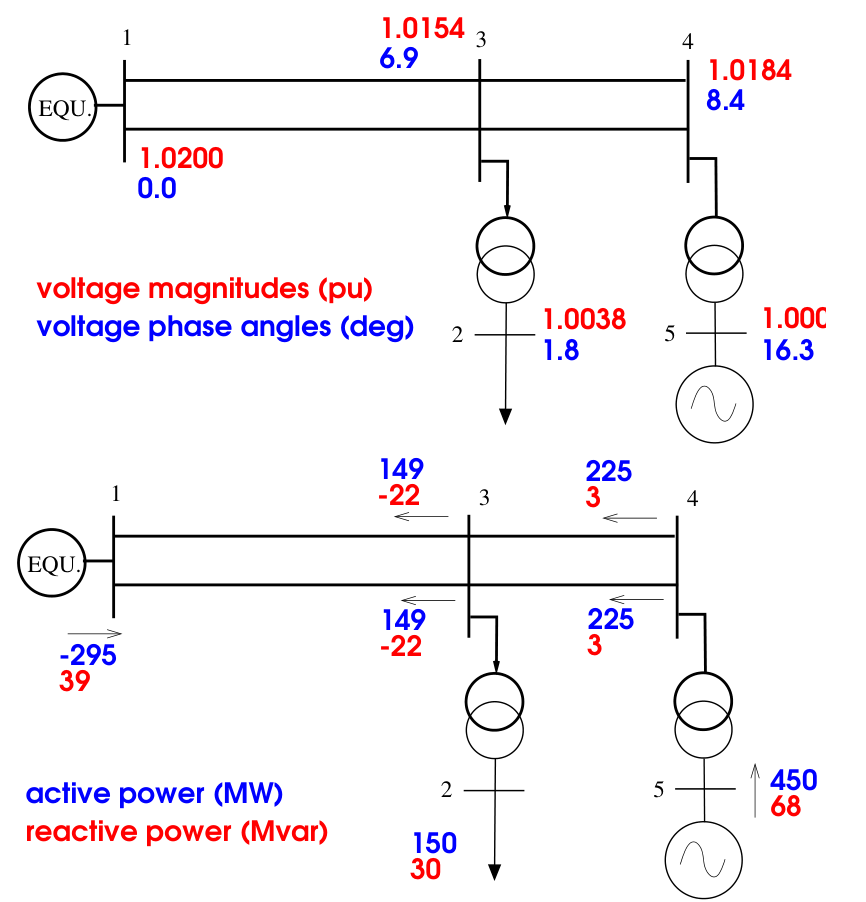
\includegraphics[width=0.9\linewidth]{OP1}
	\caption{Operating point 1}
	\label{fig:op1}
\end{figure}

\subsection{Operating point 2}

The second operating point assumes the sub-system is importing power from the grid.

\begin{figure}[H]
	\centering
	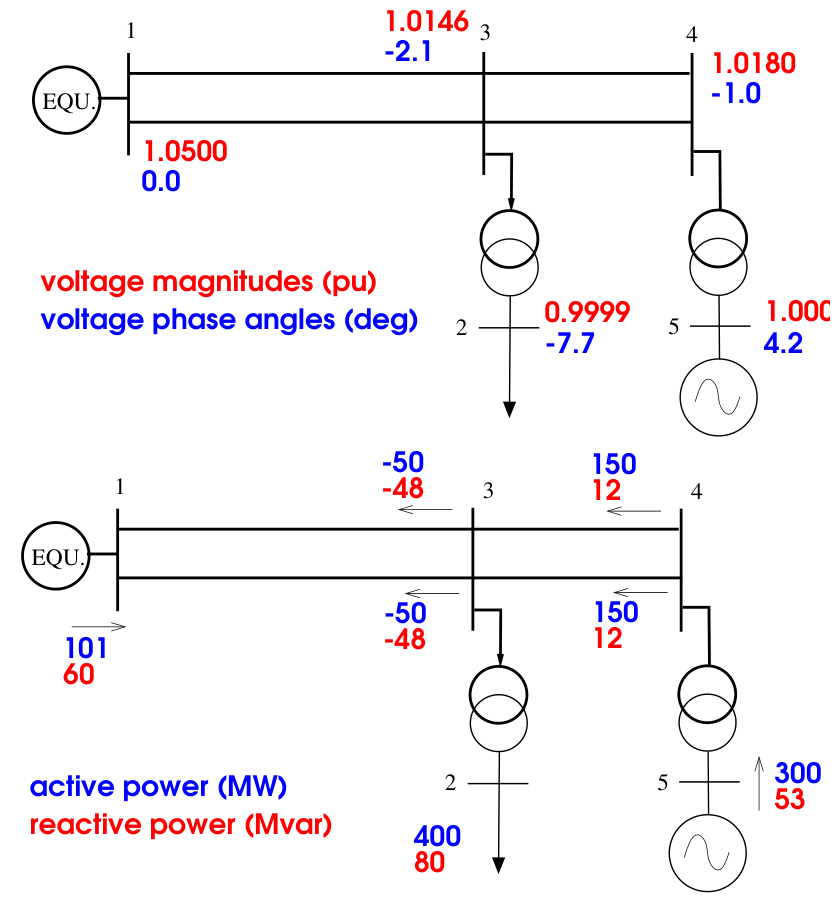
\includegraphics[width=0.9\linewidth]{OP2}
	\caption{Operating point 2}
	\label{fig:op2}
\end{figure}

\section{Syntax of disturbances}

To modify the disturbance and implement the different case studies listed below, the command \textit{addDisturb} is used:

\begin{itemize}
\item To increase the power setpoint of generator $G$ by $D$ MW in $T$ seconds: 

\textcode|ram.addDisturb($time, 'CHGPRM TOR G P0 $D MW $T')|

\item To increase the voltage setpoint of generator $G$ by D pu in T seconds: 

\textcode|ram.addDisturb($time, 'CHGPRM EXC G Vo $D $T')|

\item To increase the value of the Thévenin voltage by D pu in T seconds: 

\textcode|ram.addDisturb($time, 'CHGPRM INJ EQUIV1 ETH $D $T')|

\item To apply a fault at bus $B$ with resistance $R$ and reactance $X$ (in $\Omega$, can be zero): 

\textcode|ram.addDisturb($time, 'FAULT BUS B $R $X')|

\item To clear a fault at bus B: 

\textcode|ram.addDisturb($time, 'CLEAR BUS B')|

\item To trip line $XYZ$:

\textcode|ram.addDisturb($time, 'BREAKER BRANCH XYZ 0')|

\end{itemize}

\noindent You need to change the variables with \$ to the values required by the case studies.

\section{Syntax of observables}

To view the output after the simulation:

\begin{itemize}
	\item Generator G active power: 	
	\textcode|ext.getSync('G').P.plot()|
	
	\item Generator G reactive power: 	
	\textcode|ext.getSync('G').Q.plot()|
	
	\item Generator G frequency (in pu): 	
	\textcode|ext.getSync('G').S.plot()|
	
	\item Generator G rotor angle: 	
	\textcode|ext.getSync('G').A.plot()|
	
	\item Generator G field current: 	
	\textcode|ext.getSync('G').FC.plot()|
		
	\item Generator G valve opening: 	
	\textcode|ext.getTor('G').z.plot()|
	
	\item Generator G mechanical power: 	
	\textcode|ext.getTor('G').Pm.plot()|
	
	\item Generator G excitation control: \textcode|ext.getExc('G').dvpss.plot()|
	
	\item Generator G field voltage: 	
	\textcode|ext.getExc('G').vf.plot()|
	
	\item Bus 3 voltage magnitude:	
	\textcode|ext.getBus('3').mag.plot()|
	
	\item Bus 3 voltage magnitude:	
	\textcode|ext.getBus('3').mag.plot()|
	
	\item Load Impedance\_Load active power: 	
	\textcode|ext.getInj('Impedance_Load').P.plot()|
	
	\item Load Impedance\_Load reactive power: 	
	\textcode|ext.getInj('Impedance_Load').Q.plot()|
	
	\item Motor Large\_Motor active power: 	
	\textcode|ext.getInj('Large_Motor').P.plot()|
	
	\item Motor Large\_Motor reactive power: 	
	\textcode|ext.getInj('Large_Motor').Qmot.plot()|
	
	\item Motor Large\_Motor speed: 	
	\textcode|ext.getInj('Large_Motor').omega.plot()|
	
	\item Active power entering line 1-3: 	
	\textcode|ext.getBranch('1-3').PF.plot()|
	
	\item Rective power entering line 1-3: 	
	\textcode|ext.getBranch('1-3').QF.plot()|
	
	
\end{itemize}

\noindent You need to change the variables with \$ to the values required by the case studies.

\section{Experimental cases}

\subsection{Case 1}

Implement the following case study:
\begin{itemize}
\item  Operating point: \# 2
\item  disturbance: at $t=1 \mathrm{~s}$, increase of power set-point $P_o$ by 115 MW in 10 s
\item  simulated time: 60 s
\end{itemize}

\noindent Comment as far as possible the evolution of:
\begin{enumerate}
\item  the generator active power
\item   the generator reactive power
\item   the generator rotor angle
\item   the generator field current
\item   the control valve $z$ of the turbine
\item   the voltage magnitude at bus 3
\end{enumerate}

\subsection{Case 2}

Implement the following case study:
\begin{itemize}
\item  Operating point: \# 1
\item  disturbance: at $t=1 \mathrm{~s}$, increase of voltage set-point $V_o$ by 0.05 pu in 2 s
\item simulated time: 60 s
\end{itemize}

\noindent Comment as far as possible the evolution of:
\begin{enumerate}
\item the voltage magnitude at bus 3. In particular, explain the three "spikes" with the help of the proper curves
\item the generator active power
\item the generator reactive power
\item the generator field current.
\end{enumerate}

\subsection{Case 3}

Implement the following case study:
\begin{itemize}
\item Operating point: \#1
\item disturbance: at $t=1 \mathrm{~s}$, "voltage dip" in the external system simulated by a decrease of the Thévenin voltage by 0.20 pu during 0.04 s (can be considered as an impulse response)
\item simulated time: 20 s
\end{itemize}

\noindent Comment as far as possible the evolution of:
\begin{enumerate}
\item Observe the evolution of the rotor speed of the generator
\item Observe the evolution of the PSS output (select: generator G - observable of excitation control - dvpss)
\item take the Power System Stabilizer (PSS) out of service, simulate the same disturbance and compare the evolution of the rotor speed with the previous one
\item observe the evolution of the voltage magnitude at bus 3 and comment on the similarity
\item what is the period of the dominant oscillation?
	
\end{enumerate}

\noindent \textbf{Put the PSS back in service before proceeding!}

\subsection{Case 4}

Implement the following case study:
\begin{itemize}
\item Operating point: \#1
\item disturbance: at $t=1 \mathrm{~s}$, a solid fault on line 1-3, cleared after 4 cycles $(0.08 \mathrm{~s})$ by opening the faulted circuit. The fault takes place very near bus 3, so that it can be applied at bus 3
\item simulated time: 20 s
\end{itemize}

\noindent Comment as far as possible the evolution of:
\begin{enumerate}
\item the terminal voltage of the generator
\item the active and reactive powers of the generator
\item the rotor speed of the generator
\item the field voltage of the generator (select: generator G - observable of excitation control - vf)
\item the active power consumed by the impedance load at bus 2
\item the active power consumed by one of the motors at bus 2
\item the speed of one the motors at bus 2
\item From RAMSES outputs, determine the current in line 3-4 during the short-circuit. Consider the value just after fault occurrence, for security. Check this value with a simple circuit calculation involving the generator equivalent circuit.
\end{enumerate}

\subsection{Case 5}

Implement the following case study:
\begin{itemize}
\item Operating point: \#2
\item disturbance: at $t=1 \mathrm{~s}$, tripping of both circuits of line 1-3 (without fault)
\item simulated time: 25 s
\end{itemize}

\noindent Comment as far as possible the evolution of:
\begin{enumerate}
\item rotor speed of G
\item active power produced by G
\item control valve opening (select: generator G - observable of torque controller - z)
\item turbine mechanical power (select: generator G - observable of torque controller - Pm ; in pu on the turbine nominal power).	
\item Compute the final rotor speed using a formula from primary frequency control. Comment on the accuracy and try improving it.
\end{enumerate}



\subsection{Case 6}

Implement the following case study:
\begin{itemize}
\item Operating point: \#2
\item disturbance: at $t=1 \mathrm{~s}$, a solid fault on line 1-3, cleared after 10 cycles $(0.20 \mathrm{~s})$ by opening the faulted circuit. The fault takes place very near bus 3, so that it can be applied at bus 3
\item simulated time: 20 s 
\end{itemize}

\noindent Comment as far as possible the evolution of:
\begin{enumerate}
\item Observe that the voltage at bus 3 does not recover near 1 pu, but stays "locked" near $0.84 \mathrm{pu}$. Find which system component is responsible for this, with the help of the proper curves
\item show that for some shorter fault duration (i.e. smaller than 0.20 s), the voltage does not stay "locked" at such a small value. Explain the underlying instability mechanism.	
\end{enumerate}

\subsection{Case 7}

Implement the following case study:
\begin{itemize}
\item Operating point: $\# 1$
\item disturbance: at $t=1 \mathrm{~s}$, severe disturbance in the external system simulated by a decrease of the Thévenin voltage by 0.2 pu in 1 s (the voltage remains at its low value)
\item simulated time: 120 s
\end{itemize}

\noindent Comment as far as possible the evolution of:
\begin{enumerate}
\item Explain why the voltage at bus 3 drops so much after some time.
\end{enumerate}


\end{document}




